
%(BEGIN_QUESTION)
% Copyright 2006, Tony R. Kuphaldt, released under the Creative Commons Attribution License (v 1.0)
% This means you may do almost anything with this work of mine, so long as you give me proper credit

Denne P\&ID-en viser hvordan to trykktransmittere kan kobles med en radarnivåtransmitter for å gi data nødvendig for å beregne ikke bare væskenivå, men også væsketetthet og total væskemasse i tanken:

$$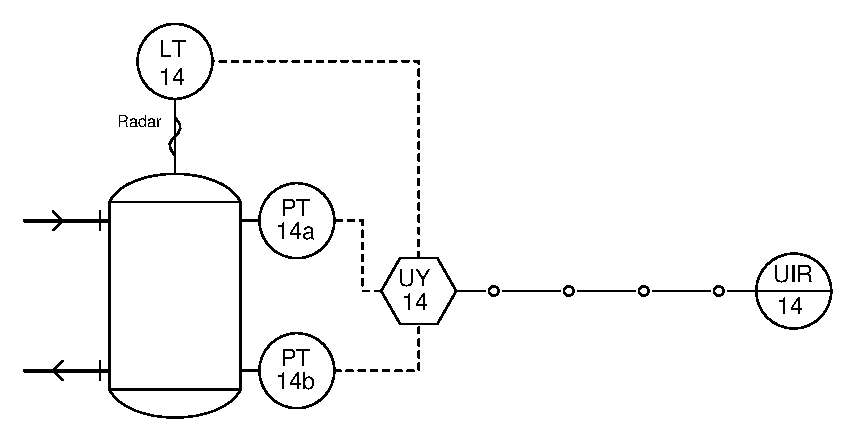
\includegraphics[width=15.5cm]{i00295x01.eps}$$

Dette kalles noen ganger et \textit{hybrid} nivåmålesystem.  Forklar hva ``hybrid'' betyr i denne sammenhengen, og hvordan de tre transmitterene oppnår målemålene for nivå, tetthet og total masse.  Forklar også hva alle symbolene betyr i P\&ID-en.

\vskip 10pt

\underbar{file i00295}
%(END_QUESTION)





%(BEGIN_ANSWER)

Bruk av to trykktransmittere, én i bunnen og én i toppen, minner om et \textit{hydrostatisk tank expert}-system (med tre trykksensorer).  Hvis tanken var ventilert, kunne vi klart oss med bare én trykktransmitter sammen med radarmåleren for å beregne nivå, tetthet og total masse.

%(END_ANSWER)





%(BEGIN_NOTES)

En tilleggseffekt av å kombinere to helt ulike nivåteknologier (radar + hydrostatisk) er redundans.  Hvis én sensor feiler, kan den andre fortsatt levere data nyttig for å bestemme prosessnivået.  Nivådatamaskinen (UY-14) kan programmeres til å ``stemme'' mellom sensorene ved avvikende målinger.

%INDEX% Measurement, level: radar + hydrostatic

%(END_NOTES)
